\documentclass{standalone}
\begin{document} 
\section{Übung 4}
\subsection{Aufgabe 4.1}
\paragraph{Ungleichungen}
Bei Ungleichungen unterscheidet man zwischen der strikten Ungleichung ($<$ und $>$) und der nicht strikten- (oder normalen) Ungleichung ($\leqslant$ und $\geqslant$).
\paragraph{Rechenregeln für Ungleichungen}
Ungleichungen können (meistens) wie Gleichungen umgeformt werden. Ausnahmen:
\begin{itemize}
\item Bei der Multiplikation und Division mit einer negativen Zahl wird das Vergleichszeichen umgedreht. 
\item Beim Quadrieren müssen beide Seiten größer als null sein
\end{itemize}
Ungleichungssysteme können mit wie Gleichungssysteme durch Addition/Multiplikation beider Seiten gelöst werden. Wenn
$a < c$ und $b < d \Rightarrow a+b < c + d$ Falls $a, b > 0$, dann gilt ebenfalls: $ab < cd$ \\
\paragraph{Rechenregeln für Betragsfunktionen}
\begin{itemize}
\item Dreiecksungleichung: $|a + b| \leqslant |a| + |b|$
\item $|a - b| \leqslant |a| + |b|$
\item Inversive Dreiecksungleichung: $||a| - |b|| \leqslant |a - b|$
\item $||a| - |b|| \leqslant |a + b|$
\item $|ab| = |a| * |b|$
\end{itemize}
\paragraph{Grafisches Lösen von Ungleichungen}
Beispiel:
$0 < y < 2x$ Alle Punkte über 0 und unter $2x$ sind Lösungen dieser Ungleichung \\
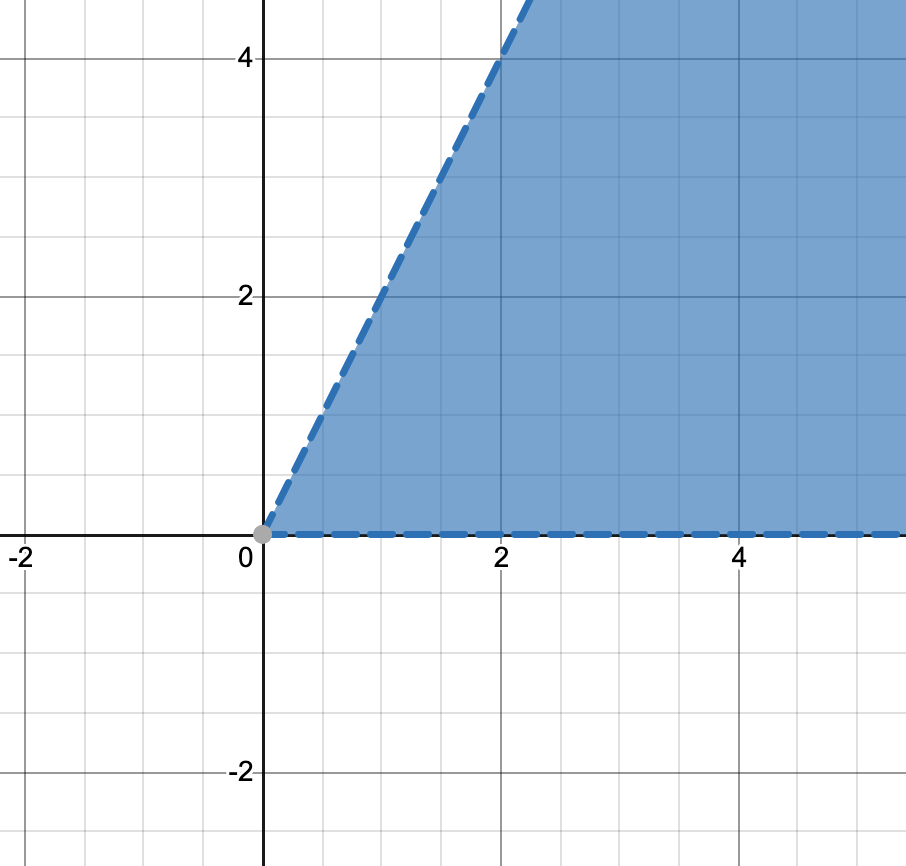
\includegraphics[width=6cm]{img/4_1.png}
\subsection{Aufgabe 4.2}
% Hier eure Lösung eingeben
\begin{itemize}
\item[a)]
$5x - 4 < 3x -1$ \\
$2x < 3$ \\
$x < \frac{3}{2}$ \\
$\mathbb{L} = ]-\infty; 1,5[$

\item[b)]
$-\frac{3}{2}(x-5) < 7$ \\
$-\frac{3}{2} x + 7,5 < 7$ \\
$-\frac{3}{2}x < -0,5 $ \\
$x > \frac{1}{3}$ \\
$\mathbb{L} = ]\frac{1}{3}; +\infty[$

\item[c)]
1. Fall: $x > 0$ \\
$x \geqslant \frac{1}{3}$\\
$\mathbb{L}_1 = [\frac{1}{3}; \infty [$ \\
2. Fall: $ x < 0$ \\
$x \leqslant \frac{1}{3}$ \\
$\mathbb{L}_2 = ]-\infty; 0[$

\item[d)]
1. Fall: $4x + 5 > 0 (\Rightarrow x > -\frac{5}{4})$ \\
$2-3x > 2x + 2,5$ \\
$5x < -0,5$ \\
$x < -\frac{1}{10}$\\
$\mathbb{L}_1 = ]-\frac{5}{4}; -\frac{1}{10}[$ \\
2. Fall: $4x + 5 < 0 (\Rightarrow x < -\frac{5}{4})$ \\
$2-3x < 2x + 2,5$ \\
$-0,5 < 5x$ \\
$-\frac{1}{10} < x$
$\mathbb{L}_2 = \{\}$

\end{itemize}
\end{document}